% Construction : la courbe de f et sa tangente au point d'abscisse a = 2,2.
% f(x) = 0,3x² + 0,4 ; f(a) = 1,852 et f'(a) = 1,32.
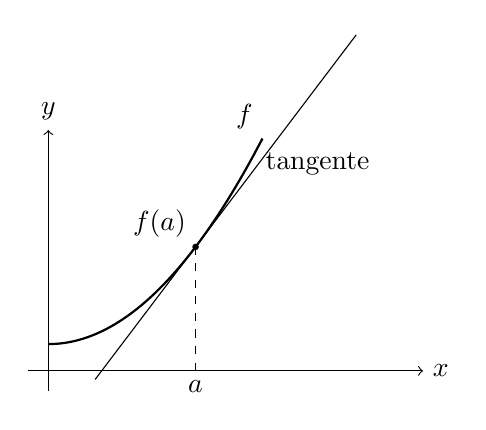
\begin{tikzpicture}[scale=0.85]
  \draw[->] (-0.3, 0) -- (5.6, 0) node[right] {$x$};
  \draw[->] (0, -0.3) -- (0, 3.6) node[above] {$y$};
  \draw[thick, domain=0:3.2, smooth, variable=\x] plot ({\x}, {0.3*\x*\x + 0.4});
  \draw[domain=0.7:4.6, variable=\x] plot ({\x}, {1.852 + 1.32*(\x - 2.2)});
  \draw[dashed] (2.2, 0) node[below] {$a$} -- (2.2, 1.852);
  \fill (2.2, 1.852) circle (1.4pt);
  \node[above left] at (2.2, 1.852) {$f(a)$};
  \node[right] at (4.6, 4.99) {};
  \node[above] at (4.1, 4.36) {};
  \node[below right] at (4.4, 4.75) {};
  \node[right] at (3.1, 3.1) {tangente};
  \node[above left] at (3.2, 3.47) {$f$};
\end{tikzpicture}
